% !TeX root = ../../main.tex
\section{案例七：CVE-2023-22482（Argo CD OIDC \texttt{aud} 未校验导致越权访问）}

\subsection{漏洞详解与复现}

\noindent\hangindent=2em\hangafter=1 \textbf{漏洞背景}

Argo CD 是 Kubernetes 场景中常用的声明式 GitOps 持续交付工具，提供 Web 与 API 接口供用户进行应用同步、回滚与差异审计等操作。
在企业环境中，Argo CD 常通过 OIDC 与统一身份提供方对接，由身份提供方向 Argo CD 签发包含用户身份与组信息的令牌。
在 OIDC 令牌中，\texttt{aud}（audience）声明用于标识该令牌的预期接收方。通常情况下，服务端除验证签名与发行者外，还需要校验 \texttt{aud} 是否包含本服务的受众标识，以避免将“为其他服务签发的令牌”误用到本服务上。

\textbf{CVE 描述}：CVE-2023-22482 指出 Argo CD 在部分版本中存在不恰当授权缺陷。其能够验证令牌由已配置的 OIDC 提供方签名，但未对令牌的 \texttt{aud} 声明进行校验，从而可能接受并非面向 Argo CD 的有效令牌。若同一身份提供方还为其他系统签发令牌，攻击者一旦获得其他系统的有效令牌，就可能将其用于访问 Argo CD。Argo CD 将基于令牌中的 \texttt{groups} 声明授予权限，即使这些组信息并非为 Argo CD 的授权场景设计。该问题在 \texttt{2.6.0-rc3}、\texttt{2.5.6}、\texttt{2.4.19} 与 \texttt{2.3.13} 及以上版本修复；受影响范围包含 \texttt{>= 1.8.2} 且低于上述修复版本的版本分支。

\textbf{主要成因分类}：安全逻辑缺陷 / 身份与授权校验缺失（令牌受众 \texttt{aud} 未校验导致跨受众令牌复用）。

\textbf{攻击链条描述}：该漏洞可抽象为”多受众身份提供\,$\rightarrow$\,跨受众令牌复用\,$\rightarrow$\,基于组声明的越权访问”的链条。攻击者获得同一 OIDC 提供方为其他受众签发的有效令牌；将其提交给 Argo CD 的接口；若 Argo CD 未校验 \texttt{aud}，则会接受该令牌并根据 \texttt{groups} 映射授予权限，进而造成对应用资源与交付流程的非预期访问。该缺陷同时放大了令牌泄露事件的影响范围。

\noindent\hangindent=2em\hangafter=1 \textbf{漏洞复现（验证性复现）}

本文采用\textbf{验证性复现}思路，验证“\texttt{aud} 不匹配的有效令牌是否会被 Argo CD 接受”这一关键安全性质。
复现过程不展开可直接复用的令牌获取与请求构造细节，而以配置证据、令牌声明证据与接口返回结果为主：在受影响版本中，若 Argo CD 在已验签前提下接受 \texttt{aud} 不匹配的令牌并返回受 RBAC 控制的资源，则可判定存在受众校验缺失；升级至修复版本后，同样令牌应在校验阶段被拒绝。完整的环境准备、验证判据与回归检查步骤见附录\ref{app:cve-2023-22482}。

\begin{figure}[htb]
	\centering
	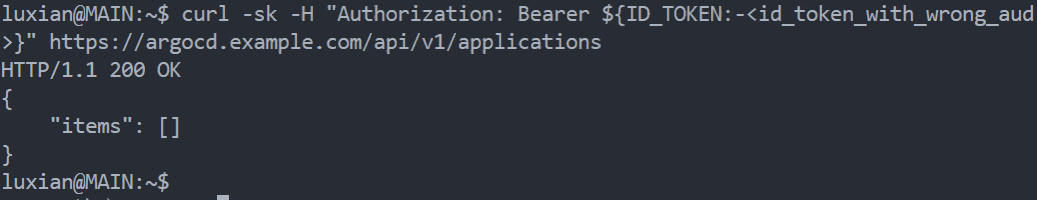
\includegraphics[width=0.8\textwidth]{images/cve7/image.png}
	\bicaption{验证性复现证据示意（审计/接口响应截图的经处理摘要）}{Illustration of validation-oriented reproduction evidence based on processed summaries of audit and API response screenshots}
	\label{fig:cve-2023-22482-evidence}
\end{figure}

\subsection{策略部署}

该漏洞的治理重点是\textbf{降低跨系统令牌复用的可行性与后果}。
在补丁窗口期内，可通过身份提供方配置、前置网关校验与 RBAC 收敛构建补偿控制，压制攻击路径并降低风险暴露面。

\textbf{策略概述}：第一，在身份提供方侧为 Argo CD 配置独立客户端与唯一受众，限制该客户端签发的组声明范围，避免与其他系统的组命名空间混用。第二，在 Argo CD 前置入口实施令牌受众强制校验，例如通过 API 网关对 \texttt{iss}、\texttt{aud} 与签名进行一致性验证，拒绝 \texttt{aud} 不匹配的请求。第三，收敛 Argo CD 的 RBAC 与项目边界，限制高权限组的授予范围，并将关键操作纳入审计与告警，降低令牌误用后的爆炸半径。
策略配置要点与验证建议见附录\ref{app:cve-2023-22482}。

\subsection{三因素分析}

\noindent\textbf{有效性（Effectiveness）：}
身份提供方侧的客户端隔离可减少可被复用的令牌来源，前置网关的 \texttt{aud} 强制校验可在应用层之前阻断异常令牌进入。RBAC 与项目边界收敛则用于限制误用令牌的权限上限，三者形成互补的纵深防御。

\noindent\textbf{无干扰性（Interference）：}
前置网关校验对访问路径有一定侵入性，需评估对 CLI、Web 与自动化流水线的影响并提供灰度策略。身份提供方的客户端隔离与组声明裁剪可能影响既有用户组映射，需要配套变更沟通与回滚预案。RBAC 收敛可能降低自助交付效率，应通过标准化角色与审批流程平衡安全与效率。

\noindent\textbf{可部署性（Deployability）：}
身份提供方侧配置与网关校验可作为平台能力复用，在多集群场景中可模板化推广。RBAC 与项目边界策略可通过 GitOps 管理并持续审计，形成长期的基线治理闭环。
